\documentclass[11pt]{article}
\usepackage[T1]{fontenc}
\usepackage{lmodern}
\usepackage[margin=1.05in]{geometry}
\usepackage{amsmath,amssymb,amsthm,mathtools}
\usepackage{microtype}
\usepackage{enumitem}
\usepackage{tikz}
\usetikzlibrary{arrows.meta,positioning,calc}
\usepackage[hidelinks]{hyperref}
\hypersetup{pdftitle={Strong Ulam Stability Characterizes Amenability},pdfauthor={OpenAI}}
\numberwithin{equation}{section}
\newtheorem{theorem}{Theorem}[section]
\newtheorem{proposition}[theorem]{Proposition}
\newtheorem{lemma}[theorem]{Lemma}
\newtheorem{corollary}[theorem]{Corollary}
\theoremstyle{definition}
\newtheorem{definition}[theorem]{Definition}
\theoremstyle{remark}
\newtheorem{remark}[theorem]{Remark}
\newcommand{\norm}[1]{\left\lVert#1\right\rVert}
\newcommand{\abs}[1]{\left\lvert#1\right\rvert}
\newcommand{\ip}[2]{\left\langle#1,#2\right\rangle}
\newcommand{\id}{I}
\newcommand{\tr}{\operatorname{Tr}}
\newcommand{\defect}{\operatorname{def}}
\newcommand{\U}{\mathcal U}
\newcommand{\E}{\mathsf E}
\newcommand{\F}{\mathsf F}
\newcommand{\cX}{\mathcal X}
\newcommand{\cY}{\mathcal Y}
\newcommand{\cH}{\mathcal H}
\newcommand{\cC}{\mathcal C}
\newcommand{\cI}{\mathcal I}
\newcommand{\Prob}{\mathbb P}
\DeclareMathOperator{\dist}{dist}
\title{Strong Ulam Stability Characterizes Amenability}
\author{OpenAI}
\date{October 5, 2026}
\begin{document}
\maketitle
\begin{abstract}
A countable discrete group is amenable if and only if it is strongly Ulam
stable: every sufficiently accurate unitary almost representation, on any
complex Hilbert space, is uniformly close in operator norm to a genuine
representation on the same space. We prove the converse to Kazhdan's
amenable stability theorem, answering the question of Burger, Ozawa, and
Thom. The inclusion of infinite-dimensional Hilbert spaces is essential.
\end{abstract}
\section{Introduction}\label{sec:introduction}

Let $G$ be a countable discrete group and let $H$ be a complex Hilbert space.
For a map $\mu:G\to\U(H)$ with $\mu(e)=I$, put
\[
 \defect(\mu)=\sup_{g,h\in G}\norm{\mu(gh)-\mu(g)\mu(h)}.
\]
The group is \emph{strongly Ulam stable} if, for every $\varepsilon>0$, there
is $\delta>0$ such that every such map with $\defect(\mu)\le\delta$ is within
$\varepsilon$, uniformly on $G$, of a unitary representation on the same
space $H$. All norms are operator norms. The number $\delta$ must work
simultaneously for all Hilbert spaces, including infinite-dimensional ones.

A group is amenable if $\ell^\infty(G)$ admits a positive linear functional
$m$ with $m(1)=1$ and $m(L_gf)=m(f)$, where $(L_gf)(x)=f(g^{-1}x)$.
Our main result is the following characterization.

\begin{theorem}\label{thm:main}
A countable discrete group is strongly Ulam stable if and only if it is
amenable.
\end{theorem}

Kazhdan proved the implication from amenability to strong Ulam stability
\cite{Kazhdan}; see also \cite[Theorems~3.1 and~3.2]{BurgerOzawaThom}.
We prove the converse. More precisely, for every
nonamenable countable group and every $\delta>0$, we construct a separable
Hilbert space $H$ and a normalized map $\mu:G\to\U(H)$ with
$\defect(\mu)<\delta$ such that
\begin{equation}\label{eq:distance-goal}
 \sup_{g\in G}\norm{\mu(g)-\rho(g)}>\frac1{10}
 \quad\text{for every unitary representation }\rho:G\to\U(H).
\end{equation}

\subsection*{History and context}
The uniform stability problem asks whether an approximate homomorphism
can be corrected without losing uniform control over the group.
Kazhdan's 1982 theorem supplies this correction for amenable groups; his
work also gives unstable almost representations of fundamental groups
of closed orientable surfaces of genus at least two
\cite{Kazhdan,BurgerOzawaThom}. Burger, Ozawa, and Thom proved that every
group containing a nonabelian free subgroup fails strong Ulam stability
\cite[Theorem~1.2]{BurgerOzawaThom}. They explicitly asked whether strong
Ulam stability characterizes amenability \cite[p.~111]{BurgerOzawaThom}.
Alpeev subsequently proved instability for restricted wreath products
$A\wr G$ when $A$ is a nontrivial countable abelian group and $G$ is
countable and nonamenable \cite[Theorem~B]{Alpeev}. His use of measured
equivalence relations reaches examples without nonabelian free subgroups.

The inclusion of infinite-dimensional Hilbert spaces is essential.
The term \emph{Ulam stability}, without ``strong'', commonly denotes the
uniform statement restricted to finite-dimensional unitary groups
\cite[Definition~2.1]{BurgerOzawaThom}. Nonamenable groups can satisfy
that property. Glebsky, Lubotzky, Monod, and Rangarajan developed
asymptotic cohomology and proved finite-dimensional stability for broad
classes of higher-rank lattices \cite{GlebskyLubotzkyMonodRangarajan}.
Fournier-Facio and Rangarajan applied this theory to wreath products over
infinite amenable groups and to Thompson groups
\cite[Theorems~1.2 and~1.3]{FournierFacioRangarajan}. These results concern
a different stability property. The failure of the corresponding
wreath-product statement for strong stability is explained in
\cite[Remark~6.1]{FournierFacioRangarajan}.

\subsection*{The construction}
The proof starts with a nontrivial minimal strongly proximal action of $G$
on a compact space, supplied by Furstenberg's boundary theory
\cite{Furstenberg,KalantarKennedy}. From this action we obtain finite choices of steps in
$G$, each marked $\E$ or $\F$ at every possible departure point. The marks
have two opposing counting properties: all but a small proportion of
steps from a fixed point are $\E$, whereas all but a small proportion
of steps ending at a fixed point are $\F$.
They also satisfy a compatibility condition along paths: an $\E$ step
can never be followed by an $\F$ step.

We use these paths to construct a Hilbert space $H$ with finitely many
levels and a copy at each group element. Fix a set $\cC$ of at most three
translated markings. For each $p\in\cC$, a unitary circuit $W_p^{\cC}$
exchanges selected subspaces of successive levels, using edges whose flags
differ within $\cC$ and whose flag in $p$ is $\F$.
For a fixed set $\cC$, the comparisons
$W_q^{\cC}(W_p^{\cC})^{-1}$ compose exactly. In constructing $\mu$, however,
each comparison uses its own pair of markings. The defect estimate
therefore requires a bound on how a comparison changes when a third
marking is added. After obtaining that bound, we compose pair comparisons
with the usual translation representation to define $\mu$.

The main analytic issue is that the two subspaces exchanged at one step
have naturally identified coordinates with slightly different inner products.
Summing the resulting errors over all layers would give no useful bound.
We instead choose the isometry between these inner products
to be almost the coordinate identity on the subspace used by the next
layer. The change caused by a third marking can then be moved past that
layer. After this move, the principal errors act on mutually orthogonal
levels, so their norms combine by a maximum rather than a sum.
Lemma~\ref{lem:priority} isolates the isometry construction, and
Proposition~\ref{prop:comparison} gives the resulting circuit estimate.
Both estimates are independent of the dimensions of the finite coordinate
spaces.

The obstruction to a genuine representation is a quadratic form. We use
two orthonormal bases with opposite signs and a family of anticommuting
involutions. The signed basis sums force the form to vanish on vectors
obtained from any genuine representation. The initial inner product of
our construction makes the same form equal to $1/2$. Most of the labelled
paths transport the final vectors back to these initial vectors, producing
the fixed distance bound~\eqref{eq:distance-goal}.

Section~\ref{sec:flags} constructs the marks. Section~\ref{sec:linear}
proves the finite-dimensional estimates and the metric-transfer lemmas.
Sections~\ref{sec:construction} and~\ref{sec:comparison} construct the
circuits and control their dependence on the markings.
Section~\ref{sec:obstruction} proves the quadratic-form obstruction and
chooses the parameters.

\subsection*{Conventions}
Inner products are conjugate-linear in the first argument. On a coordinate
space with a positive matrix $A$, the notation $(V,A)$ means the inner
product $\ip{u}{v}_A=u^*Av$. Unless a metric is indicated, a matrix norm is
Euclidean. Metrics between $\frac12 I$ and $2I$ make these norms uniformly
equivalent. A numerical constant $C$ may increase from one occurrence to
the next; it never depends on the group, the number of labels, or the
number of levels. We write an explicit factor $N$ whenever an estimate
sums over $N$ levels.

\section{Flags from a boundary action}\label{sec:flags}

We first convert nonamenability into finite families of labelled steps in
$G$.  Each step will carry a flag $\E$ or $\F$.  The construction makes $\F$
rare when a departure is fixed and $\E$ rare when an arrival is fixed.
At the same time, an $\E$ step prevents every outgoing step at the next
stage from having flag $\F$.  This last property will allow common parts
of two circuits to cancel exactly.

A compact $G$-space is a \emph{boundary} if its action is minimal and
strongly proximal: every orbit is dense, and the weak-star closure of
the orbit of every Radon probability measure contains a point mass.
We use the standard boundary characterization of amenability: a
nonamenable discrete group admits a non-singleton compact Hausdorff
boundary \cite{Furstenberg}; see also
\cite[Section~3]{KalantarKennedy}. Fix such a boundary $K$.
Minimality implies that the orbit closure of any probability contains
\emph{every} point mass once it contains one.

The space $K$ has no isolated points.  Indeed, if it had an isolated
point, minimality would imply that all its points are isolated, so
compactness would make $K$ finite.  The uniform probability on $K$ is
invariant, contradicting strong proximality unless $K$ is a singleton.
Consequently, every nonempty open subset of $K$ contains arbitrarily
many pairwise disjoint nonempty open subsets.

The following consequence of strong proximality provides the finite
lists used at each stage.  The requirement at the distinguished point
$\zeta$ is what makes the stages compatible.

\begin{lemma}[Uniform lists with a prescribed point]\label{lem:uniform-list}
Let $K$ be a compact Hausdorff boundary, let $U\subseteq K$ be nonempty
and open, let $\zeta\in K$, and let $0<\beta<1$.  There is a finite
nonempty list $s_1,\ldots,s_M\in G$, with repetitions allowed, such that
\[
 s_j^{-1}\zeta\in U\quad(1\leq j\leq M),
 \qquad
 \frac{1}{M}\#\{j:s_j^{-1}t\notin U\}<\beta
 \quad(t\in K).
\]
Moreover, some open neighborhood $O$ of $\zeta$ satisfies
$s_j^{-1}O\subseteq U$ for every $j$.
\end{lemma}

\begin{proof}
Choose $t_0\in U$ and a continuous function $f:K\to[0,1]$ with
$f(t_0)=1$ and support contained in $U$.  Consider the family
\[
 \mathcal A=\{f\circ s^{-1}:s\in G,\ s^{-1}\zeta\in U\}
 \subset C(K,\mathbb R).
\]
For every Radon probability $m$ on $K$, there is $a\in\mathcal A$ with
\begin{equation}\label{eq:boundary-integral}
 \int_K a\,dm>1-\frac{\beta}{2}.
\end{equation}
To see this, apply strong proximality and minimality to
$\nu=(m+\delta_\zeta)/2$.  Since $\delta_{t_0}$ belongs to the orbit
closure of $\nu$, some $s\in G$ satisfies
\[
 \frac12\left(\int_K f(s^{-1}t)\,dm(t)
                      +f(s^{-1}\zeta)\right)>1-\frac{\beta}{4}.
\]
Both terms in parentheses are at most one, so each exceeds
$1-\beta/2$.  In particular, $s^{-1}\zeta\in U$, which proves
\eqref{eq:boundary-integral}.

We claim that the convex hull of $\mathcal A$ contains a function
strictly larger than $1-\beta$ everywhere.  Otherwise, separate that
convex hull from the nonempty open convex set
\[
 \mathcal O=\{q\in C(K,\mathbb R):q(t)>1-\beta\text{ for all }t\in K\}
\]
by the Hahn--Banach theorem.  There is a nonzero continuous real linear
functional $\Lambda$ such that
\[
 \sup_{a\in\mathcal A}\Lambda(a)
 \leq \inf_{q\in\mathcal O}\Lambda(q).
\]
This functional is positive.  Indeed, if $u\geq0$ and $q\in\mathcal O$,
then $q+tu\in\mathcal O$ for every $t\geq0$; the displayed separation
would be impossible if $\Lambda(u)<0$.  A nonzero positive functional
satisfies $\Lambda(1)>0$, so we may normalize it to have
$\Lambda(1)=1$.  The Riesz representation theorem then identifies
$\Lambda$ with integration against a Radon probability $m$.  Applying
the separation inequality to the constant functions
$q=1-\beta+\varepsilon$ and letting $\varepsilon\downarrow0$ gives
\[
 \sup_{a\in\mathcal A}\int_K a\,dm\leq1-\beta,
\]
contradicting \eqref{eq:boundary-integral}.

Thus a finite convex combination of functions from $\mathcal A$
exceeds $1-\beta$ on $K$.  Compactness gives a strictly positive uniform
margin.  Approximate its coefficients by nonnegative rational
coefficients summing to one, closely enough to preserve that margin.
Clearing denominators produces a list with
\[
 \frac1M\sum_{j=1}^M f(s_j^{-1}t)>1-\beta\qquad(t\in K).
\]
Because $f$ vanishes outside $U$ and takes values in $[0,1]$, this is the
required counting inequality.  Finally,
$O=\bigcap_{j=1}^M s_jU$ is an open neighborhood of $\zeta$ and has the
asserted image property.
\end{proof}

We now arrange these lists into stages.  The two labels at stage $k$
will be denoted by $x\in\mathcal X_k$ and
$y\in\mathcal Y_{k-1}$; the corresponding step is
$w\longmapsto w s_k(x,y)$.

\begin{proposition}[Compatible sparse flags]\label{prop:flags}
Let $G$ be a nonamenable discrete group.  For every integer $N\geq1$
and every $0<\beta<1$, there are finite nonempty sets
$\mathcal X_1,\ldots,\mathcal X_N$ and
$\mathcal Y_0,\ldots,\mathcal Y_{N-1}$, maps
\[
 s_k:\mathcal X_k\times\mathcal Y_{k-1}\longrightarrow G,
 \qquad
 b_k:G\times\mathcal X_k\times\mathcal Y_{k-1}
       \longrightarrow\{\E,\F\},
\]
with the following properties.
\begin{enumerate}
\item[\textup{(F1)}] If $k<N$ and $b_k(w;x,y)=\E$, then, with
$v=w s_k(x,y)$,
\[
 b_{k+1}(v;x',y')=\E
 \quad\text{for every }(x',y')\in
            \mathcal X_{k+1}\times\mathcal Y_k.
\]
\item[\textup{(F2)}] For every $k,w,x$,
\[
 \frac{\#\{y\in\mathcal Y_{k-1}:b_k(w;x,y)=\F\}}
      {|\mathcal Y_{k-1}|}\leq\beta.
\]
\item[\textup{(F3)}] For every $k,v,y$,
\[
 \frac{\#\{x\in\mathcal X_k:
          b_k(v s_k(x,y)^{-1};x,y)=\E\}}
      {|\mathcal X_k|}\leq\beta.
\]
\end{enumerate}
Each alphabet may subsequently be replaced by any positive integer
number of copies, independently of the others, while preserving these
properties.  In particular, its cardinality can be made arbitrarily
large and divisible by any prescribed positive integer.
\end{proposition}

\begin{proof}
Fix points $\xi,\zeta\in K$ and choose an integer $C>1/\beta$.
We construct nonempty open sets $U_0,\ldots,U_N$ and the stage maps
backwards, starting with $U_N=K$.

Suppose that $U_k$ is already chosen.  Inside it choose pairwise
disjoint nonempty open sets $U_{k,1},\ldots,U_{k,C}$, and set
$\mathcal X_k=\{1,\ldots,C\}$.  For each $c\in\mathcal X_k$, apply
Lemma~\ref{lem:uniform-list} to $U_{k,c}$ and the point $\zeta$.
Repeat the resulting lists to give them a common length $M_k$, and
index each list by the same set
$\mathcal Y_{k-1}=\{1,\ldots,M_k\}$.  Write its entries as $s_k(c,y)$.
Set
\[
 U_{k-1}
   =\bigcap_{c\in\mathcal X_k}\ 
      \bigcap_{y\in\mathcal Y_{k-1}}s_k(c,y)U_{k,c}.
\]
This is an open neighborhood of $\zeta$, and it satisfies
\begin{equation}\label{eq:backward-regions}
 s_k(c,y)^{-1}U_{k-1}\subseteq U_{k,c}
       \subseteq U_k\qquad(c,y).
\end{equation}
This completes the backward construction.

For a step $w\longmapsto v=w s_k(c,y)$, define
\begin{equation}\label{eq:boundary-flags}
 b_k(w;c,y)=\E
 \quad\Longleftrightarrow\quad v^{-1}\xi\in U_{k,c},
\end{equation}
and otherwise give it flag $\F$.
If this step has flag $\E$, then $v^{-1}\xi\in U_k$.
For every next-stage label $(c',y')$, equation
\eqref{eq:backward-regions} at stage $k+1$ gives
\[
 (v s_{k+1}(c',y'))^{-1}\xi
   =s_{k+1}(c',y')^{-1}v^{-1}\xi\in U_{k+1,c'}.
\]
This proves \textup{(F1)}.

For fixed $w,c$, apply the counting conclusion of
Lemma~\ref{lem:uniform-list} at the boundary point $w^{-1}\xi$.
The condition for flag $\E$ is precisely
$s_k(c,y)^{-1}w^{-1}\xi\in U_{k,c}$, so fewer than a
$\beta$ fraction of $y$ have flag $\F$.  This proves \textup{(F2)}.
For fixed $v,y$, the unique departure of the step with first label $c$
and arrival $v$ is $v s_k(c,y)^{-1}$.  Its flag is $\E$ exactly when
$v^{-1}\xi\in U_{k,c}$.  The color sets are disjoint, so at most one
of the $C$ labels has this property.  Since $1/C<\beta$, this proves
\textup{(F3)}.

Finally, replace any alphabet by its product with a finite nonempty
set and pull back the maps $s_k$ and flags $b_k$ under the coordinate
projections.  All counting proportions remain unchanged, and
\textup{(F1)} remains exact.  This proves the assertion about
cardinalities.
\end{proof}

For $g\in G$, define the translated flags $p=gb$ by
\[
 p_k(w;x,y)=b_k(g^{-1}w;x,y).
\]
A \emph{configuration} will mean such a translate.  Every
configuration satisfies \textup{(F1)--(F3)}, since left translation
carries $w\longmapsto w s_k(x,y)$ to a step with the same labels.
In particular, along any path through the successive stages, the
$\F$ steps form an initial segment: after its first $\E$ step, every
remaining step has flag $\E$.

\section{Frames and metric transfers}\label{sec:linear}

We need two kinds of linear algebra with estimates independent of dimension.
First, a union of two orthonormal bases will be almost orthonormal on every
sufficiently small set of labels; the same construction supplies symmetric
involutions with small sparse restrictions.  Second, when two inner products differ
slightly, we will choose an isometry that changes a prescribed subspace by
much less than it changes the whole space.  This second choice will prevent
errors from adding over all the levels of the construction.

All matrices in the first lemma are real; we use their complexifications
when forming Hilbert spaces.  For a finite set $E$, write $P_S$ for the
coordinate projection associated with a subset $S\subseteq E$.

\begin{lemma}[Sparse restrictions]\label{lem:sparse}
For every $0<\eta<1/4$ there is $0<\beta_0<1/16$ with the following property.
If $0<\beta\leq\beta_0$, then for every sufficiently large integer $m$
there are unit vectors $(a_x)_{x\in X}$ in $\mathbb R^m$, where
$|X|=2m$, and signs $f(x)\in\{1,-1\}$ such that:
\begin{enumerate}
\item the vectors with either sign form an orthonormal basis, and hence
\begin{equation}\label{eq:frame-cancellation}
 \sum_{x\in X} f(x)a_xa_x^*=0;
\end{equation}
\item if $S\subseteq X$ and $|S|\leq4\beta|X|$, the synthesis map
$F_S:\ell^2(S)\to\mathbb C^m$, $F_Se_x=a_x$, satisfies
\begin{equation}\label{eq:sparse-gram}
 \norm{F_S^*F_S-\id}\leq\eta.
\end{equation}
\end{enumerate}
Moreover, for every sufficiently large integer $n$ there is a real
orthogonal $n\times n$ matrix $O$ such that, on a set $Y$ of size $2n$,
\begin{equation}\label{eq:JZ}
 J=\begin{pmatrix}0&O\\ O^*&0\end{pmatrix},
 \qquad Z=\begin{pmatrix}\id&0\\0&-\id\end{pmatrix}
\end{equation}
satisfy
\begin{equation}\label{eq:sparse-J}
 \norm{P_SJP_T}\leq\eta
 \quad\text{whenever}\quad |S|,|T|\leq4\beta|Y|.
\end{equation}
In particular, $J^*=J$, $J^2=Z^2=\id$, $JZ=-ZJ$, and every diagonal
entry of $J$ is zero.
\end{lemma}

\begin{proof}
We give the elementary probabilistic argument, a standard use of
concentration for Haar orthogonal matrices; compare
\cite[Section~IV-B]{LyubarskiiVershynin}.
Let $O$ be Haar distributed on the orthogonal group of $\mathbb R^m$.
For fixed real unit vectors $u,v$, the random variable $u^*Ov$ has the
distribution of the first coordinate of a uniform point on the unit
sphere.  Represent that point as
$(g_1,\ldots,g_m)/(\sum_jg_j^2)^{1/2}$, where the $g_j$ are independent
standard Gaussians.  Conditioning on $\sum_{j=2}^m g_j^2$ and using the
Gaussian tail bound gives, for $0<t<1$,
\begin{align*}
 \mathbb P\{|u^*Ov|>t\}
 &\leq 2\,\mathbb E\exp\left(
   -\frac{t^2}{2(1-t^2)}\sum_{j=2}^m g_j^2\right)\\
 &=2(1-t^2)^{(m-1)/2}
 \leq 2\exp\bigl(-(m-1)t^2/2\bigr).
\end{align*}

Put $q=8\beta<1/2$.  For any nonempty coordinate sets $S,T$ of size at most
$q m$, take $1/4$-nets in their real unit spheres, with at most
$9^{|S|}$ and $9^{|T|}$ points.  A bilinear form whose absolute value is
at most $\eta/2$ on these nets has operator norm at most $\eta$.
Indeed, approximating each of a maximizing pair of unit vectors changes
the form by at most half its operator norm.  The number of subsets of
$\{1,\ldots,m\}$ of size at most $qm$ is at most
$\exp(mH(q))$, where
\[
 H(q)=-q\log q-(1-q)\log(1-q).
\]
Thus the probability that some such submatrix $P_SOP_T$ has norm
larger than $\eta$ is at most
\[
 2\exp\left(2mH(q)+2qm\log9-\frac{m\eta^2}{16}\right)
 \qquad(m\geq2).
\]
Choose $\beta_0$ so small that, for $q=8\beta_0$,
$2H(q)+2q\log9<\eta^2/32$.  The displayed probability is then less
than one for all sufficiently large $m$.  Hence there is an orthogonal
matrix all of whose submatrices with at most $qm$ rows and columns
have norm at most $\eta$.  Real and complex operator norms agree for
these real matrices.

Take the two bases to be the standard basis and the columns of this
matrix, with signs $+1$ and $-1$.  For a subset of their union, its Gram
matrix minus the identity has block form
\[
 \begin{pmatrix}0&O_{S,T}\\O_{S,T}^*&0\end{pmatrix}.
\]
Its norm is $\norm{O_{S,T}}$, proving
\eqref{eq:sparse-gram}.  Applying the same construction in dimension
$n$ gives \eqref{eq:JZ}.  Each restriction in
\eqref{eq:sparse-J} has two off-diagonal blocks of the preceding type;
they have orthogonal domains and orthogonal ranges, so its norm is the
larger of their norms.
\end{proof}

We will use the following consequence of \eqref{eq:sparse-gram}.
For every allowed subset $S$, symmetric orthonormalization gives the
column isometry
\begin{equation}\label{eq:symmetric-orthonormalization}
 \widetilde F_S=F_S(F_S^*F_S)^{-1/2},
 \qquad \norm{\widetilde F_S-F_S}\leq C\eta.
\end{equation}
This follows by applying the scalar bound
$|t^{-1/2}-1|\leq C|t-1|$ on $[3/4,5/4]$ to $F_S^*F_S$.
If $S\subseteq T$ and both subsets are allowed, then
$\widetilde F_S$ and the restriction of $\widetilde F_T$ to
$\ell^2(S)$ differ by at most $2C\eta$: both are within $C\eta$ of
$F_S$.  All these bounds hold for every subset simultaneously.

We next compare two inner products on the same vector space.  A positive
operator $B$ defines
$\langle x,y\rangle_B=\langle x,By\rangle$; the corresponding operator
norm is denoted by $\norm{\cdot}_B$.  The next lemma singles out a
subspace $R$ that the change of coordinates must preserve.  Preservation
here means that the map takes $R$ onto $R$; it need not preserve the
original orthogonal complement of $R$.

\begin{lemma}[Transfer with a prescribed subspace]\label{lem:priority}
Let $A,B$ be positive operators on a Hilbert space $E$ such that
\[
 \tfrac12\id\leq A,B\leq2\id,
 \qquad A-B=h\Gamma,
 \qquad \Gamma^*=\Gamma,
 \qquad \norm{\Gamma}\leq1,
 \qquad 0\leq h\leq\tfrac18.
\]
Let $P$ be an orthogonal projection commuting with $B$, set $R=PE$, and
assume $\norm{P\Gamma P}\leq\eta$, where $0\leq\eta\leq1$.
There is a specified invertible operator $S_R$ such that
\begin{equation}\label{eq:priority-estimates}
 S_R^*AS_R=B,\qquad S_R(R)=R,\qquad
 \norm{S_R-\id}\leq Ch,\qquad
 \norm{(S_R-\id)P}\leq Ch\eta.
\end{equation}
The constant $C$ is absolute, and the estimates also hold in the
$B$-norm after changing $C$.

If $R\subseteq R'$ and both projections satisfy these hypotheses, then
\begin{equation}\label{eq:nested-transfer}
 K=S_{R'}^{-1}S_R
 \quad\text{satisfies}\quad
 K^*BK=B,\qquad \norm{K-\id}_B\leq Ch,\qquad
 \norm{(K-\id)P}_B\leq Ch\eta.
\end{equation}
The construction commutes with orthogonal direct sums and with every
orthogonal projection commuting with $A$, $B$, and $P$.
\end{lemma}

\begin{proof}
First make the $B$ inner product Euclidean.  Define
\[
 \widehat A=B^{-1/2}AB^{-1/2}
   =\id+hB^{-1/2}\Gamma B^{-1/2}.
\]
Since $P$ commutes with $B$, this change of coordinates preserves
$E=R\oplus R^\perp$.  Relative to this decomposition write
\[
 \widehat A=\begin{pmatrix}a&b\\b^*&d\end{pmatrix},
 \qquad E_0=d-b^*a^{-1}b.
\]
The assumptions imply
\[
 \norm{\widehat A-\id}\leq2h,
 \qquad \norm{a-\id_R}\leq2h\eta.
\]
In particular, $a$ and the Schur complement $E_0$ are positive and
invertible.  Define
\begin{equation}\label{eq:priority-map}
 Q_R=
 \begin{pmatrix}
 a^{-1/2}&-a^{-1}bE_0^{-1/2}\\
 0&E_0^{-1/2}
 \end{pmatrix},
 \qquad S_R=B^{-1/2}Q_RB^{1/2}.
\end{equation}
The same formula applies when either summand is zero, with the empty
blocks omitted.  Multiplication gives
$Q_R^*\widehat A Q_R=\id$, and hence $S_R^*AS_R=B$.
Its first block column also shows that $S_R(R)=R$.

For completeness, the bounds are uniform even when $E$ is infinite
dimensional.  We have $a\geq(1-2h)\id_R$ and
$\norm{b}\leq2h$.  Moreover,
\[
 E_0\geq(1-2h)\id_{R^\perp},\qquad
 \norm{E_0-\id_{R^\perp}}
 \leq2h+\frac{4h^2}{1-2h}.
\]
The lower bound follows by minimizing
$\langle (x,y),\widehat A(x,y)\rangle$ over $x\in R$ for fixed $y$.
Functional calculus in these fixed spectral intervals now gives
\[
 \norm{Q_R-\id}\leq Ch,
 \qquad
 \norm{(Q_R-\id)P}
   =\norm{a^{-1/2}-\id_R}\leq Ch\eta.
\]
Conjugation by $B^{1/2}$ changes the bounds by at most a factor of two,
which proves \eqref{eq:priority-estimates}.

For nested subspaces, both $S_R$ and $S_{R'}$ are isometries from the
$B$ inner product to the $A$ inner product.  Thus $K$ is $B$-unitary.
Also
\[
 K-\id=S_{R'}^{-1}(S_R-S_{R'}).
\]
The two terms $S_R-\id$ and $S_{R'}-\id$ are $O(h)$ on $E$ and
$O(h\eta)$ on $R$, since $R\subseteq R'$.  The inverse $S_{R'}^{-1}$
has uniformly bounded norm, proving \eqref{eq:nested-transfer}.
Finally, every operation in \eqref{eq:priority-map} respects the stated
common reducing subspaces.
\end{proof}

There is also a choice of isometry from the $B$ inner product to the
$A$ inner product that does not depend on $R$:
\begin{equation}\label{eq:fixed-transfer}
 C_{A,B}=A^{-1/2}B^{1/2},\qquad C_{A,B}^*AC_{A,B}=B.
\end{equation}
It respects every common reducing subspace of $A$ and $B$.
We will use this fixed map for one direction of a unitary exchange, and
$S_R^{-1}$ for the other direction.  A unitary exchange between two
orthogonal subspaces need not be an involution.

The last lemma converts an approximately fixed subspace into an exactly
fixed one.  Its dimension-free estimate also permits orthogonal sums
over all group locations.

\begin{lemma}[Fixing a subspace exactly]\label{lem:truncate}
Let $U$ be a unitary on a Hilbert space $E$, and let $P$ be an orthogonal
projection.  Suppose
\[
 \norm{U-\id}\leq t<\tfrac12,
 \qquad \norm{(U-\id)P}\leq e\leq\tfrac12.
\]
There is a unitary $\widehat U$ that is the identity on $PE$ and leaves
$(\id-P)E$ invariant, with
\[
 \norm{\widehat U-U}\leq3e,
 \qquad \norm{\widehat U-\id}\leq t+3e.
\]
The statement holds in arbitrary Hilbert space dimension.
\end{lemma}

\begin{proof}
Relative to $E=PE\oplus(\id-P)E$, write
\[
 U=\begin{pmatrix}a&b\\c&d\end{pmatrix}.
\]
Since $(U^*-\id)P=-U^*(U-\id)P$, both $(U-\id)P$ and
$P(U-\id)$ have norm at most $e$.  In particular,
$\norm{b},\norm{c}\leq e$, and
\[
 \left\|U-\begin{pmatrix}\id&0\\0&d\end{pmatrix}\right\|
 \leq2e.
\]
The compression $d$ satisfies $\norm{d-\id}\leq t<1$, so it is
invertible even in infinite dimension.  Its polar factor
$v=d(d^*d)^{-1/2}$ is therefore unitary.  Unitarity of $U$ gives
$d^*d=\id-b^*b$, whence
\[
 \norm{v-d}
 =\norm{\id-(d^*d)^{1/2}}
 \leq1-\sqrt{1-e^2}\leq e^2.
\]
Taking $\widehat U=\id\oplus v$ proves
$\norm{\widehat U-U}\leq2e+e^2\leq3e$.
The remaining estimate follows by the triangle inequality.
\end{proof}

Lemma~\ref{lem:truncate} also applies to the $B$ inner product in
Lemma~\ref{lem:priority}: a projection commuting with $B$ remains
orthogonal for that inner product.

\section{Hilbert spaces and unitary circuits}\label{sec:construction}

We now turn the flags of Proposition~\ref{prop:flags} into unitary circuits.
The circuits will move vectors between levels while replacing one
orthonormal coordinate factor at a time by a redundant frame. The inner
products are chosen so that these replacements accumulate a detectable
change between the first and last levels.

\subsection{Labels and inner products}
Fix an integer $L$, put $N=L+1$, and set
\begin{equation}\label{eq:h}
 h=\frac1{2\sqrt L}.
\end{equation}
We take $L$ larger than the numerical lower bounds required below.
In particular, $h\le1/8$ as in Lemma~\ref{lem:priority}.
Let $\eta>0$ be small and choose $\beta>0$
as in Lemma~\ref{lem:sparse}. Proposition~\ref{prop:flags} supplies the
alphabets and flags for $N$ stages. By repeating labels, we may arrange
that all alphabets have sufficiently large even cardinality for
Lemma~\ref{lem:sparse} to apply. Repetition preserves the three flag
properties.

Write $\abs{\cX_k}=2m_k$. For $x\in\cX_k$, let
$a_{k,x}\in\mathbb R^{m_k}$ be the union of two orthonormal bases, and
write $f_k(x)=1$ or $-1$ according to its basis. In particular,
\begin{equation}\label{eq:signed-frame}
 \sum_{x\in\cX_k}f_k(x)a_{k,x}a_{k,x}^*=0.
\end{equation}
For $1\le d\le L$, let $J_d$ and $Z_d$ be the matrices supplied by
Lemma~\ref{lem:sparse} on $\mathbb R^{\cY_d}$. Thus $J_d$ is a symmetric
involution, has zero diagonal, and anticommutes with the diagonal parity
matrix $Z_d$. All coordinate spaces will be complexified.

The set of full labels is
\[
 \cI=\prod_{k=1}^N\cX_k\times\prod_{d=0}^L\cY_d.
\]
Coordinates of $i\in\cI$ are written $x_k(i),y_d(i)$. On the formal
orthonormal label space $\mathbb C^{\cI}$ define
\begin{equation}\label{eq:clifford}
 \gamma_d=f_d(X_d)Z_1\cdots Z_{d-1}J_d,
 \qquad D=\frac1{\sqrt L}\sum_{d=1}^L\gamma_d.
\end{equation}
This uses the Jordan--Wigner parity-string construction
\cite{JordanWigner}; see also \cite[Section~6]{BravyiKitaev}.
We check the anticommutation relations directly.
Here $f_d(X_d)$ denotes the diagonal operator on the $\cX_d$ factor,
and each $Z_j,J_j$ acts on its indicated $\cY_j$ factor; omitted factors
carry the identity. If $d<e$, the factors $J_d$ and $Z_d$ cause
$\gamma_d\gamma_e=-\gamma_e\gamma_d$, while all other relevant factors
commute. Hence
\begin{equation}\label{eq:D-identities}
 \gamma_d^* =\gamma_d,\qquad \gamma_d^2=I,\qquad
 D^*=D,\qquad D^2=I,\qquad \tr D=0.
\end{equation}
The last identity follows from the zero diagonal of every $J_d$.

For $0\le k\le N$, let the coordinate space at level $k$ be
\[
 E_k=\bigotimes_{j\le k}\mathbb C^{m_j}
      \otimes\bigotimes_{j>k}\mathbb C^{\cX_j}
      \otimes\bigotimes_{d=0}^L\mathbb C^{\cY_d}.
\]
On $E_k$ the expression for $\gamma_d$ still makes sense whenever $d>k$:
its $\cX_d$ coordinate has not been replaced by a frame. Set
\begin{equation}\label{eq:level-metric}
 G_k=I+h\sum_{k<d\le L}\gamma_d.
\end{equation}
Anticommutation gives
\begin{equation}\label{eq:metric-bound}
 \frac12 I\le G_k\le\frac32 I,
 \qquad G_0=I+\frac12D,\qquad G_L=G_N=I.
\end{equation}
The label vector $v_i^{(k)}\in E_k$ uses $a_{j,x_j(i)}$ in factors $j\le k$,
the standard vector $e_{x_j(i)}$ in factors $j>k$, and $e_{y_d(i)}$ in every
$\cY_d$ factor. Its $G_k$-norm is one: every added term in
\eqref{eq:level-metric} has zero diagonal in some $\cY_d$ factor.

We will repeatedly use two features of $G_k$. It is the identity on the
compressed factors $\mathbb C^{m_j}$, $j\le k$. It commutes with each
coordinate projection in $\cX_j$ for $j>k$ and in $\cY_d$ for $d\le k$.
For the latter assertion, a term surviving in~\eqref{eq:level-metric}
contains only diagonal parity operators on those $\cY_d$ factors.

Take the Hilbert direct sum
\begin{equation}\label{eq:big-space}
 H=\bigoplus_{k=0}^N\ \bigoplus_{w\in G}(E_k,G_k),
 \qquad H_k=\bigoplus_{w\in G}(E_k,G_k).
\end{equation}
It is separable. Left translation of the location $w$ defines a genuine
unitary representation $U:G\to\U(H)$. No translation changes a label or
a level.

\subsection{The subspaces exchanged by one layer}
Fix a nonempty set $\cC$ of at most three configurations, and $p\in\cC$.
The use of sets allows repeated translates to be removed without changing
any definition. A stage-$k$ edge is a quadruple $(w,k,x,y)$, with arrival
$v=ws_k(x,y)$. It is \emph{switchable for $\cC$} if its flags are not the
same in all configurations of $\cC$.
The layer for $p$ will exchange exactly the switchable edges flagged $\F$
in $p$. We first choose their endpoint subspaces simultaneously for all
$p\in\cC$.

At a fixed arrival $v$ and fixed $y\in\cY_{k-1}$, put
\begin{equation}\label{eq:switchable-set}
 S_{k,v,y}^{\cC}=
 \{x\in\cX_k:\ (vs_k(x,y)^{-1},k,x,y)
                 \text{ is switchable for }\cC\}.
\end{equation}
Every switchable edge is flagged $\E$ in some configuration. By the
arrival bound (F3),
\begin{equation}\label{eq:switchable-size}
 \abs{S_{k,v,y}^{\cC}}\le\abs{\cC}\beta\abs{\cX_k}.
\end{equation}
Let $F_S:\mathbb C^S\to\mathbb C^{m_k}$ have columns $a_{k,x}$,
$x\in S=S_{k,v,y}^{\cC}$. Replace these columns by
\begin{equation}\label{eq:adjusted-frame}
 \widetilde F_S=F_S(F_S^*F_S)^{-1/2},
 \qquad \widetilde a_{k,v,y,x}^{\cC}=\widetilde F_Se_x.
\end{equation}
The sparse Gram estimate makes this well-defined and gives
\begin{equation}\label{eq:frame-adjustment}
 \widetilde F_S^*\widetilde F_S=I,
 \qquad \norm{\widetilde F_S-F_S}\le C\eta.
\end{equation}
For $S=\varnothing$ there are no columns to adjust.

The left subspace of a switchable edge is the coordinate sector at
$(k-1,w)$ with $X_k=x$ and $Y_{k-1}=y$. Its right subspace, at $(k,v)$,
has $Y_{k-1}=y$ and $X_k$ in the line spanned by
$\widetilde a_{k,v,y,x}^{\cC}$. Every other tensor factor is unrestricted.
For distinct edges these left subspaces are orthogonal; so are these
right subspaces. On the right this uses~\eqref{eq:adjusted-frame} and the
fact that $G_k$ is the identity on the compressed $X_k$ factor.

Both endpoint subspaces have the same residual coordinates after removing
the fixed $X_k$ and $Y_{k-1}$ factors. Their metrics, denoted $A_{x,y}$ on
the left and $B_y$ on the right, are the corresponding restrictions of
$G_{k-1}$ and $G_k$. For $k\le L$,
\begin{equation}\label{eq:edge-metrics}
 A_{x,y}=B_y+h\Gamma_{x,y},\qquad
 \Gamma_{x,y}=f_k(x)Z_1\cdots Z_{k-1}J_k\big|_{Y_{k-1}=y},
 \qquad \norm{\Gamma_{x,y}}=1.
\end{equation}
The right metric $B_y$ is independent of $x$. Earlier compressed $X$
factors carry identity operators throughout. At $k=N$ both metrics are
identity.

\subsection{Metric transfer with priority for the next layer}
For $k\le L$, arrival $v$, and next coordinate $z\in\cX_{k+1}$, define
\begin{equation}\label{eq:priority-set}
 R_{k,v,z}^{\cC}=
 \{t\in\cY_k:\ q_{k+1}(v;z,t)=\F
                         \text{ for some }q\in\cC\}.
\end{equation}
The row bound (F2) gives $\abs{R_{k,v,z}^{\cC}}\le3\beta\abs{\cY_k}$.
Let $P_{k,v}^{\cC}$ be the residual-coordinate projection that, in the
sector $X_{k+1}=z$, selects $Y_k\in R_{k,v,z}^{\cC}$. It is the identity
on all remaining factors.

This projection commutes with $B_y$. Moreover,
\begin{equation}\label{eq:compressed-gamma}
 \norm{P_{k,v}^{\cC}\Gamma_{x,y}P_{k,v}^{\cC}}\le\eta.
\end{equation}
Indeed, decompose by the future $X$ coordinates and earlier $Y$
coordinates. In each block the compression is, up to a sign and identity
factors, a compression $J_k[R,R]$ with $\abs R\le3\beta\abs{\cY_k}$.
Lemma~\ref{lem:sparse} applies. Taking a direct sum does not increase
the bound.

Apply Lemma~\ref{lem:priority} to obtain a specified isometry
\[
 S_e^{\cC}:(\text{residual coordinates},B_y)
                  \longrightarrow(\text{residual coordinates},A_{x,y})
\]
for this edge. In the original coordinates it satisfies
\begin{equation}\label{eq:edge-transfer}
 \norm{S_e^{\cC}-I}\le Ch,\qquad
 \norm{(S_e^{\cC}-I)P_{k,v}^{\cC}}\le Ch\eta.
\end{equation}
At $k=N$ put $S_e^{\cC}=I$. We will use $(S_e^{\cC})^{-1}$ for the
left-to-right part of the exchange. For its right-to-left part, use the
fixed isometry
\begin{equation}\label{eq:fixed-leg}
 C_{x,y}=A_{x,y}^{-1/2}B_y^{1/2}:(B_y)\longrightarrow(A_{x,y}).
\end{equation}
It is independent of $\cC$, $p$, and the priority projection.

On the left and right subspaces of an edge, in that order, define
\begin{equation}\label{eq:swap}
 M_e^{\cC}=
 \begin{pmatrix}0&C_{x,y}\\(S_e^{\cC})^{-1}&0\end{pmatrix}.
\end{equation}
Both off-diagonal entries are isometries onto the indicated endpoint, so
$M_e^{\cC}$ is unitary. In general it is not an involution. The distinction
is useful: its inverse takes a vector from the right to the left using
$S_e^{\cC}$, whereas its forward right-to-left block is $C_{x,y}$.

The stage-$k$ layer $M_{p,k}^{\cC}$ applies~\eqref{eq:swap} on every
switchable edge flagged $\F$ in $p$, and is identity on the orthogonal
complement of their endpoint subspaces. The orthogonality proved above
makes this a unitary, even when infinitely many locations occur. Define
\begin{equation}\label{eq:circuit}
 W_p^{\cC}=M_{p,N}^{\cC}\cdots M_{p,1}^{\cC},
 \qquad V_{qp}^{\cC}=W_q^{\cC}(W_p^{\cC})^{-1}.
\end{equation}
Thus layers are applied in the order $1,\ldots,N$.

Every recipe uses coordinate projections and positive square roots, and
depends on group locations only through the flags. Consequently
\begin{equation}\label{eq:equivariance}
 U(g)W_p^{\cC}U(g)^{-1}=W_{gp}^{g\cC},
 \qquad U(g)V_{qp}^{\cC}U(g)^{-1}=V_{gq,gp}^{g\cC}.
\end{equation}
This is the covariance needed to turn the pairwise comparisons into an
almost representation. The next section establishes that introducing a
third configuration changes those comparisons only slightly.

\section{Comparing two and three configurations}\label{sec:comparison}

Inside one fixed set $\cC$, the comparisons compose exactly:
$V_{rq}^{\cC}V_{qp}^{\cC}=V_{rp}^{\cC}$. For the almost representation,
however, each comparison will be made using its own pair of configurations.
We therefore need the following estimate.

\begin{proposition}\label{prop:comparison}
There are numerical constants $C$ and $h_0>0$ such that, for the construction
of Section~\ref{sec:construction} with $h\le h_0$ and $0<\eta\le1/4$,
\begin{equation}\label{eq:comparison}
 \norm{V_{qp}^{\{p,q\}}-V_{qp}^{\{p,q,r\}}}
 \le Ch+CN\eta+CNh\eta
\end{equation}
for every three configurations $p,q,r$. The constants do not depend on
the cardinalities of any alphabets or on the configurations.
\end{proposition}

The proof has three parts. We first put both constructions in the same
arrival frames. Extra exchanges common to $p$ and $q$ then cancel exactly.
The remaining change is in the priority isometries. Their small errors can
be moved to separate levels instead of being summed along a path.

\subsection{Changing the arrival frames}
Write $\cC_2=\{p,q\}$ and $\cC_3=\{p,q,r\}$. At each arrival sector,
$S_2=S_{k,v,y}^{\cC_2}\subset S_3=S_{k,v,y}^{\cC_3}$. By
\eqref{eq:frame-adjustment},
\begin{equation}\label{eq:two-frame-distance}
 \norm{\widetilde F_{S_2}-\widetilde F_{S_3}|_{\mathbb C^{S_2}}}
 \le C\eta.
\end{equation}
For the moment, replace the pair's arrival vectors by the corresponding
columns of $\widetilde F_{S_3}$, leaving its edges and priorities unchanged.
Denote the resulting layers by $\overline M_{p,k}$ and circuit by
$\overline W_p$; define $\overline W_q$ in the same way.

We justify the operator-norm cost without summing over columns. For one
layer, let $L$ and $R$ be the isometric embeddings of the direct sums of
its active left and right residual spaces into $H$. Let $T$ be the direct
sum of its left-to-right transfers, and $C_0$ the direct sum of the fixed
right-to-left transfers. The layer equals
\begin{equation}\label{eq:layer-embedding}
 I-LL^*-RR^*+LC_0R^*+RTL^*.
\end{equation}
Only $R$ changes when the arrival frame changes. Its domain uses the
metric $B_y$ on each column, independent of the compressed coordinate
$X_k$. Thus~\eqref{eq:two-frame-distance}, tensored with the residual
coordinates and summed orthogonally over $(v,y)$, gives
$\norm{R-R'}\le C\eta$. Formula~\eqref{eq:layer-embedding} then bounds
the layer change by $4\norm{R-R'}$. The transfers have norm one in their
respective metrics, even though they may depend on the column $x$.
It follows by telescoping products of unitaries that
\begin{equation}\label{eq:frame-circuit-cost}
 \norm{W_p^{\cC_2}-\overline W_p}\le CN\eta,
 \qquad \norm{W_q^{\cC_2}-\overline W_q}\le CN\eta.
\end{equation}

\subsection{Cancelling the common exchanges}
Among edges switchable for $\cC_3$ but not for $\cC_2$, those flagged $\E$
in both $p$ and $q$ are unused by both circuits. The others are flagged
$\F$ in both and are exchanged by both circuits with exactly the same
unitary. Call these the common exchanges.

A common exchange in a later layer commutes with every noncommon exchange
in an earlier layer. Only adjacent layers could share a level. If the
earlier edge is noncommon and is used in one of the two circuits, it is
$\E$ in one of $p,q$. By (F1), at its arrival location there is no outgoing
$\F$ edge in that configuration at the next stage. A later common exchange
there is therefore impossible. Their supports at the shared level lie
at disjoint group locations. The adjustment of the $X$ vectors changes
no location and hence preserves this disjointness.

Within a layer all exchanges commute, being supported on orthogonal
subspaces. We may therefore move all common exchanges to the beginning
of each circuit, retaining their relative order. There are only finitely
many layers; infinite families within a layer are orthogonal direct sums,
so this rearrangement does not require an infinite product. We obtain
\begin{equation}\label{eq:common-cancel}
 W_p^{\cC_3}=\widehat W_p C_{\mathrm{com}},\qquad
 W_q^{\cC_3}=\widehat W_q C_{\mathrm{com}},\qquad
 V_{qp}^{\cC_3}=\widehat W_q\widehat W_p^{-1}.
\end{equation}
Here $\widehat W_p=\widehat M_{p,N}\cdots\widehat M_{p,1}$ consists
of the pair-switchable edges used by $p$, with the triple's frames and
priorities. Thus $\widehat M_{p,k}$ and $\overline M_{p,k}$ now have the
same edges, subspaces, and fixed reverse transfers. Only their priority
isometries differ.

\subsection{Moving the priority changes past later layers}
We compare $\widehat W_p$ with $\overline W_p$; the argument for $q$ is
identical. For each active edge the smaller priority projection is
contained in the larger one. From~\eqref{eq:swap},
\[
 \begin{pmatrix}0&C_{x,y}\\(S_e^{\cC_3})^{-1}&0\end{pmatrix}
 \begin{pmatrix}0&S_e^{\cC_2}\\C_{x,y}^{-1}&0\end{pmatrix}
 =\begin{pmatrix}I&0\\0&(S_e^{\cC_3})^{-1}S_e^{\cC_2}\end{pmatrix}.
\]
Consequently
\begin{equation}\label{eq:post-unitary}
 \widehat M_{p,k}=K_k\overline M_{p,k},
 \qquad K_k|_{H_k^\perp}=I,\qquad \norm{K_k-I}\le Ch.
\end{equation}
These norms are in $H$, with its given metric. The last estimate follows
from Lemma~\ref{lem:priority} and the uniform metric bounds.

For $k<N$, let $Q_{k+1}$ be the orthogonal projection onto the departure
subspace used by $\overline M_{p,k+1}$ in $H_k$. We claim that
\begin{equation}\label{eq:next-protected}
 \norm{(K_k-I)Q_{k+1}}\le Ch\eta.
\end{equation}
At a fixed location, $Q_{k+1}$ selects the next coordinates $X_{k+1},Y_k$.
A current arrival subspace selects $Y_{k-1}$ and a line in the compressed
$X_k$ factor. These projections commute: the conditions concern different
coordinates, and $G_k$ preserves the indicated coordinate sectors.
On their intersection the smaller priority contains every next departure,
by~\eqref{eq:priority-set}. Lemma~\ref{lem:priority} bounds
$(S_e^{\cC_3})^{-1}S_e^{\cC_2}-I$ there by $Ch\eta$. On the complement
of all current arrival subspaces $K_k=I$. Their orthogonal direct sum proves
\eqref{eq:next-protected}; no factor counting edges or labels occurs.
Set $Q_{N+1}=0$ for the last layer.

Apply Lemma~\ref{lem:truncate} on $H_k$, taking $h_0$ sufficiently small.
It gives a unitary $\widetilde K_k$, extended by identity off $H_k$, such
that
\begin{equation}\label{eq:corrected-unitary}
 \widetilde K_kQ_{k+1}=Q_{k+1},\qquad
 \norm{K_k-\widetilde K_k}\le Ch\eta,\qquad
 \norm{\widetilde K_k-I}\le Ch.
\end{equation}
It commutes with $\overline M_{p,k+1}$: that layer acts only on its
departure subspace $Q_{k+1}H_k$ and its arrival subspace in $H_{k+1}$,
and $\widetilde K_k$ is identity on both. It also commutes with all later
layers, which act on other levels. Figure~\ref{fig:priority} depicts the
only later layer whose support overlaps $H_k$.

\begin{figure}[t]
\centering
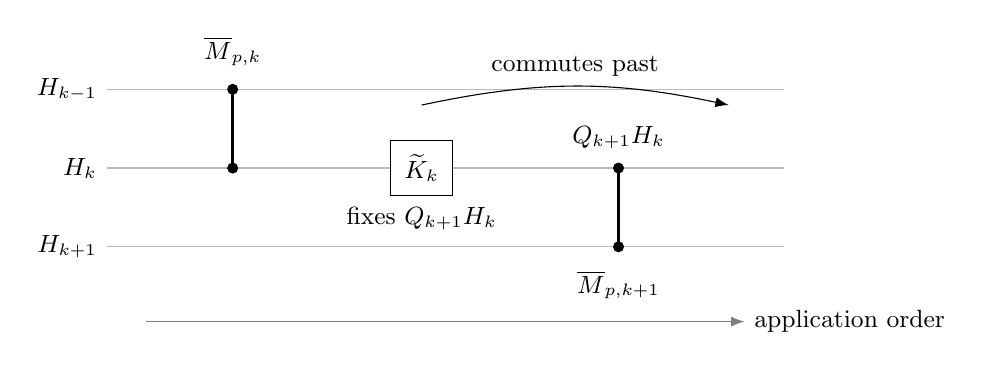
\begin{tikzpicture}[x=1cm,y=1cm,>=Latex,font=\small]
 \foreach \y/\lab in {2/{H_{k-1}},1/{H_k},0/{H_{k+1}}}{
   \draw[gray!55] (0,\y)--(8.6,\y);
   \node[left] at (0,\y) {$\lab$};
 }
 \draw[very thick] (1.6,1)--(1.6,2);
 \fill (1.6,1) circle (2pt);\fill (1.6,2) circle (2pt);
 \node[above] at (1.6,2.18) {$\overline M_{p,k}$};
 \node[draw,fill=white,inner sep=5pt] (corr) at (4,1) {$\widetilde K_k$};
 \node[below=2pt of corr,fill=white,inner sep=2pt] {fixes $Q_{k+1}H_k$};
 \draw[very thick] (6.5,0)--(6.5,1);
 \fill (6.5,0) circle (2pt);\fill (6.5,1) circle (2pt);
 \node[below] at (6.5,-.18) {$\overline M_{p,k+1}$};
 \node[above] at (6.5,1.12) {$Q_{k+1}H_k$};
 \draw[->] (4,1.8) to[bend left=12] node[above]{commutes past} (7.9,1.8);
 \draw[->,gray] (.5,-.95)--(8.1,-.95) node[right,black]{application order};
\end{tikzpicture}
\caption{The corrected priority change acts only at level $k$ and fixes
the next layer's departure subspace $Q_{k+1}H_k$. It therefore commutes past
that layer. All subsequent layers have support disjoint from $H_k$. Horizontal
lines denote orthogonal levels; vertical segments indicate layers acting
between successive levels.}
\label{fig:priority}
\end{figure}

Substitute~\eqref{eq:post-unitary} into the product for $\widehat W_p$.
Replacing each $K_k$ by $\widetilde K_k$ costs at most $CNh\eta$ by
telescoping. Move every $\widetilde K_k$ past the subsequent layers.
The corrected unitaries commute with one another because they act on
distinct levels. Thus
\begin{equation}\label{eq:moved-errors}
 \norm{\widehat W_p-
    (\widetilde K_N\cdots\widetilde K_1)\overline W_p}
 \le CNh\eta,
 \qquad
 \norm{\widetilde K_N\cdots\widetilde K_1-I}
 =\max_k\norm{\widetilde K_k-I}\le Ch.
\end{equation}
Together with~\eqref{eq:frame-circuit-cost}, this proves
\[
 \norm{\widehat W_p-W_p^{\cC_2}}\le Ch+CN\eta+CNh\eta,
\]
and the same bound holds for $q$. Using~\eqref{eq:common-cancel} and
telescoping the two factors in $V_{qp}$ proves
Proposition~\ref{prop:comparison}.

\subsection{The almost representation}
Return to the original configuration $b$ and define
\begin{equation}\label{eq:mu}
 \mu(g)=V_{b,gb}^{\{b,gb\}}U(g).
\end{equation}
When $g=e$, there is just one configuration and no switchable edge;
therefore $\mu(e)=I$. Equivariance~\eqref{eq:equivariance} gives
\[
 \mu(g)\mu(t)
 =V_{b,gb}^{\{b,gb\}}V_{gb,gtb}^{\{gb,gtb\}}U(gt).
\]
Replace both comparisons here and the comparison in $\mu(gt)$ by those
computed in $\{b,gb,gtb\}$. Within that common set,
\[
 V_{b,gb}^{\{b,gb,gtb\}}V_{gb,gtb}^{\{b,gb,gtb\}}
 =V_{b,gtb}^{\{b,gb,gtb\}}.
\]
Three applications of Proposition~\ref{prop:comparison} yield
\begin{equation}\label{eq:defect-bound}
 \defect(\mu)\le Ch+CN\eta+CNh\eta.
\end{equation}
The remaining task is to show that the distance from representations
does not tend to zero with this bound.

\section{Distance from genuine representations}\label{sec:obstruction}

The map $\mu$ has small defect by~\eqref{eq:defect-bound}. To separate it
from genuine representations, we compare labelled vectors at the last
and first levels. Most labels are transported between these vectors by
$\mu$, but a quadratic form takes incompatible values on the two families
if that transport is performed by a genuine representation.

\subsection{Transport along most paths}
For $i\in\cI$, abbreviate $s_k(i)=s_k(x_k(i),y_{k-1}(i))$ and put
\[
 t_0(i)=e,\qquad t_k(i)=s_1(i)\cdots s_k(i),\qquad s_i=t_N(i).
\]
Let $u_i$ be $v_i^{(N)}$ at location $e$ and level $N$, and let $r_i$ be
$v_i^{(0)}$ at location $e$ and level zero. Both are unit vectors.

\begin{lemma}\label{lem:transport}
For all but a proportion $2N\beta$ of labels $i\in\cI$,
\begin{equation}\label{eq:transport-bound}
 \norm{\mu(s_i)u_i-r_i}\le CN\eta+CNh\eta.
\end{equation}
\end{lemma}

\begin{proof}
Give $\cI$ its uniform product probability measure. Along the forward
path $t_0,\ldots,t_N$, the departure $t_{k-1}$ depends only on coordinate
pairs $(X_j,Y_{j-1})$ with $j<k$. Conditional on these pairs and on $X_k$,
the coordinate $Y_{k-1}$ is still uniform. The row bound (F2) therefore
makes the probability of an $\F$ step at most $\beta$. A union bound shows
that every forward step is $\E$ with probability at least $1-N\beta$.

Consider also the path with the same steps and terminal point $e$. Its
stage-$k$ arrival is
\begin{equation}\label{eq:backward-position}
 a_k(i)=s_N(i)^{-1}s_{N-1}(i)^{-1}\cdots s_{k+1}(i)^{-1}
       =s_i^{-1}t_k(i).
\end{equation}
Thus $a_{k-1}s_k=a_k$, and $a_k$ depends only on the later coordinate pairs.
Conditional on these pairs and $Y_{k-1}$, the arrival bound (F3) makes the
probability of an $\E$ step at most $\beta$. Every backward-path step is
$\F$ with probability at least $1-N\beta$.

Let $\cI_{\mathrm{good}}$ be the intersection of these two events. We have
\begin{equation}\label{eq:good-fraction}
 \abs{\cI\setminus\cI_{\mathrm{good}}}/\abs{\cI}\le2N\beta.
\end{equation}
No independence between the two events is needed. For $i$ in this set,
put $p=s_i b$. Equation~\eqref{eq:backward-position} and the definition
of translation show that the forward path $t_0,\ldots,t_N$ is entirely
$\E$ for $b$ and entirely $\F$ for $p$. All its edges are switchable for
$\{b,p\}$.

Let $z_k$ be the exact label vector $v_i^{(k)}$ at location $t_k(i)$.
Thus $z_N=U(s_i)u_i$ and $z_0=r_i$. At stage $k$, replacing its factor
$a_{k,x_k(i)}$ by the adjusted arrival vector changes $z_k$ by at most
$C\eta$, by~\eqref{eq:frame-adjustment} and~\eqref{eq:metric-bound}.
The adjusted vector belongs to the active right subspace of the path's
edge. The inverse layer takes it to the left using $S_e^{\{b,p\}}$.
For $k<N$, its residual coordinates belong to the priority subspace:
the next step $(t_k,x_{k+1},y_k)$ is $\F$ in $p$.
Equation~\eqref{eq:edge-transfer} therefore changes these coordinates by
at most $Ch\eta$. At $k=N$ the transfer is identity. We conclude that
\[
 \norm{(M_{p,k}^{\{b,p\}})^{-1}z_k-z_{k-1}}
 \le C\eta+Ch\eta.
\]
Telescoping the inverse circuit from $N$ to $1$ gives
\[
 \norm{(W_p^{\{b,p\}})^{-1}U(s_i)u_i-r_i}
 \le CN\eta+CNh\eta.
\]
All actual layers are unitary, so the previously incurred errors are not
amplified. Finally $W_b^{\{b,p\}}r_i=r_i$: its first layer does not use
the departure sector of the first, $\E$-flagged step, and later layers
do not act on level zero. Formula~\eqref{eq:mu} proves the claim.
\end{proof}

\subsection{A quadratic form that vanishes for representations}
The signed frames were chosen to make the following identity hold for
every genuine representation, without any assumption that it preserve
our tensor factors or levels.

\begin{lemma}\label{lem:witness}
Let $\rho:G\to\U(H)$ be a unitary representation, and define unit vectors
in $\mathbb C^{\cI}\otimes H$ by
\[
 \psi=\abs{\cI}^{-1/2}\sum_{i\in\cI}e_i\otimes\rho(s_i)u_i,
 \qquad
 r=\abs{\cI}^{-1/2}\sum_{i\in\cI}e_i\otimes r_i.
\]
Then
\begin{equation}\label{eq:witness-values}
 \ip{\psi}{(D\otimes I)\psi}=0,
 \qquad \ip{r}{(D\otimes I)r}=\frac12.
\end{equation}
In particular, $\norm{r-\psi}\ge1/4$.
\end{lemma}

\begin{proof}
For any labels $i,j$, unitarity and multiplicativity give
\[
 \ip{\rho(s_i)u_i}{\rho(s_j)u_j}
 =\ip{u_i}{\rho(s_i^{-1}s_j)u_j}.
\]
Fix $d\in\{1,\ldots,L\}$. A nonzero coefficient $(\gamma_d)_{ij}$
pairs labels that agree except possibly in $Y_d$. Their group products
have a common prefix through stage $d$:
\[
 s_i=P Q_i,\qquad s_j=P Q_j,
 \qquad s_i^{-1}s_j=Q_i^{-1}Q_j.
\]
After all coordinates other than $X_d$ are fixed, the suffixes $Q_i,Q_j$
are independent of $X_d$: steps after $d$ use only $X_{d+1},\ldots,X_N$.
There are linear isometric embeddings $E_i,E_j:\mathbb C^{m_d}\to H$,
also independent of $X_d$, such that
$u_i=E_i a_{d,x_d}$ and $u_j=E_j a_{d,x_d}$. Here the metric at level
$N$ is Euclidean. The factor of $(\gamma_d)_{ij}$ that depends on $X_d$
is exactly $f_d(x_d)$. Consequently the sum over that coordinate is a
fixed scalar multiple of
\begin{align*}
 &\sum_{x\in\cX_d} f_d(x)
   \ip{a_{d,x}}{E_i^*\rho(Q_i^{-1}Q_j)E_j a_{d,x}}\\
 &\hspace{1cm}=
 \tr\left(E_i^*\rho(Q_i^{-1}Q_j)E_j
        \sum_{x\in\cX_d}f_d(x)a_{d,x}a_{d,x}^*\right)=0
\end{align*}
by~\eqref{eq:signed-frame}. Summing all other coordinates proves
$\ip{\psi}{(\gamma_d\otimes I)\psi}=0$, and summing $d$ proves the
first identity in~\eqref{eq:witness-values}.

The Gram matrix of the vectors $r_i$ is $G_0$, since these are the standard
label vectors at level zero. Both $G_0$ and $D$ are real symmetric.
Equations~\eqref{eq:D-identities} and~\eqref{eq:metric-bound} give
\[
 \ip{r}{(D\otimes I)r}
 =\frac{\tr(DG_0)}{\abs{\cI}}
 =\frac{\tr(D+\frac12D^2)}{\abs{\cI}}=\frac12.
\]
Since $\norm D=1$ and both vectors have norm one,
\[
 \frac12
 \le \norm{r-\psi}\norm r+\norm\psi\norm{r-\psi}
 =2\norm{r-\psi}.
\]
This proves the last assertion.
\end{proof}

\subsection{Parameter choice and the main theorem}
Suppose that $\rho$ is uniformly within $\varepsilon$ of $\mu$.
Lemma~\ref{lem:transport} bounds the transport error on
$\cI_{\mathrm{good}}$; on its complement the error is at most two,
because both vectors are unit. The triangle inequality in the orthogonal
label sum therefore gives
\begin{equation}\label{eq:final-distance}
 \norm{r-\psi}
 \le \varepsilon+CN\eta+CNh\eta+2\sqrt{2N\beta}.
\end{equation}
All constants in this estimate and~\eqref{eq:defect-bound} are numerical.
We can now make the parameter order explicit.

\begin{proof}[Proof of Theorem~\ref{thm:main}]
The amenable implication is Kazhdan's theorem~\cite{Kazhdan}.
Suppose that $G$ is nonamenable, and fix any $\delta>0$.
First choose $L$ large enough that $h=1/(2\sqrt L)$ meets every numerical
smallness condition above and $Ch<\delta/2$ in~\eqref{eq:defect-bound}.
With $N=L+1$ now fixed, choose $0<\eta<1/4$ so small that
\[
 CN\eta+CNh\eta<\min\{\delta/2,1/20\}
\]
for the constants in both~\eqref{eq:defect-bound} and
\eqref{eq:final-distance}. Next choose
\[
 0<\beta<\min\{\beta_0(\eta),\,1/(3200N)\},
\]
where $\beta_0(\eta)$ is supplied by Lemma~\ref{lem:sparse}.
Construct the flags and then enlarge the alphabets to the dimensions
required by that lemma. None of the established estimates worsens when
the alphabets are enlarged.

The resulting normalized map has defect less than $\delta$.
If a genuine representation were uniformly within $1/10$ of it,
\eqref{eq:final-distance} would give
\[
 \norm{r-\psi}<\frac1{10}+\frac1{20}+\frac1{20}=\frac15,
\]
contrary to Lemma~\ref{lem:witness}. Thus~\eqref{eq:distance-goal} holds
for every $\delta>0$, which rules out strong Ulam stability.
\end{proof}

\begin{thebibliography}{10}
\raggedright
\bibitem{Alpeev}
A.~Alpeev,
\emph{Lamplighters over non-amenable groups are not strongly Ulam stable},
\href{https://arxiv.org/abs/2009.11738v3}{arXiv:2009.11738} (2020), version~3, 2023.

\bibitem{BravyiKitaev}
S.~Bravyi and A.~Kitaev,
\emph{Fermionic quantum computation},
Ann. Physics \textbf{298} (2002), no.~1, 210--226.
\href{https://doi.org/10.1006/aphy.2002.6254}{doi:10.1006/aphy.2002.6254}.

\bibitem{BurgerOzawaThom}
M.~Burger, N.~Ozawa, and A.~Thom,
\emph{On Ulam stability},
Israel J. Math. \textbf{193} (2013), 109--129.
\href{https://doi.org/10.1007/s11856-012-0050-z}{doi:10.1007/s11856-012-0050-z}.

\bibitem{FournierFacioRangarajan}
F.~Fournier-Facio and B.~Rangarajan,
\emph{Ulam stability of lamplighters and Thompson groups},
Math. Ann. \textbf{389} (2024), 2469--2497.
\href{https://doi.org/10.1007/s00208-023-02708-5}{doi:10.1007/s00208-023-02708-5}.

\bibitem{Furstenberg}
H.~Furstenberg,
\emph{Boundary theory and stochastic processes on homogeneous spaces},
in \emph{Harmonic Analysis on Homogeneous Spaces},
Proc. Sympos. Pure Math. \textbf{26}, Amer. Math. Soc., Providence, RI,
1973, 193--229.

\bibitem{GlebskyLubotzkyMonodRangarajan}
L.~Glebsky, A.~Lubotzky, N.~Monod, and B.~Rangarajan,
\emph{Asymptotic cohomology and uniform stability for lattices in semisimple groups},
\href{https://arxiv.org/abs/2301.00476v4}{arXiv:2301.00476}, version~4 (2023).

\bibitem{JordanWigner}
P.~Jordan and E.~Wigner,
\emph{{\"U}ber das Paulische {\"A}quivalenzverbot},
Z. Phys. \textbf{47} (1928), 631--651.
\href{https://doi.org/10.1007/BF01331938}{doi:10.1007/BF01331938}.

\bibitem{KalantarKennedy}
M.~Kalantar and M.~Kennedy,
\emph{Boundaries of reduced $C^*$-algebras of discrete groups},
J. reine angew. Math. \textbf{727} (2017), 247--267.
\href{https://doi.org/10.1515/crelle-2014-0111}{doi:10.1515/crelle-2014-0111}.

\bibitem{Kazhdan}
D.~Kazhdan,
\emph{On $\varepsilon$-representations},
Israel J. Math. \textbf{43} (1982), no.~4, 315--323.
\href{https://doi.org/10.1007/BF02761236}{doi:10.1007/BF02761236}.

\bibitem{LyubarskiiVershynin}
Y.~Lyubarskii and R.~Vershynin,
\emph{Uncertainty principles and vector quantization},
IEEE Trans. Inform. Theory \textbf{56} (2010), no.~7, 3491--3501.
\href{https://doi.org/10.1109/TIT.2010.2048458}{doi:10.1109/TIT.2010.2048458}.
\end{thebibliography}

\end{document}
